%%%%%%%%%%%%%%%%%%%%%%% file typeinst.tex %%%%%%%%%%%%%%%%%%%%%%%%%
%
% This is the LaTeX source for the instructions to authors using
% the LaTeX document class 'llncs.cls' for contributions to
% the Lecture Notes in Computer Sciences series.
% http://www.springer.com/lncs       Springer Heidelberg 2006/05/04
%
% It may be used as a template for your own input - copy it
% to a new file with a new name and use it as the basis
% for your article.
%
% NB: the document class 'llncs' has its own and detailed documentation, see
% ftp://ftp.springer.de/data/pubftp/pub/tex/latex/llncs/latex2e/llncsdoc.pdf
%
%%%%%%%%%%%%%%%%%%%%%%%%%%%%%%%%%%%%%%%%%%%%%%%%%%%%%%%%%%%%%%%%%%%


\documentclass[runningheads,a4paper]{llncs}

\usepackage{amssymb}
\usepackage[utf8]{inputenc}
\usepackage[english]{babel}
\usepackage{minted}
\usemintedstyle{colorful}
\setcounter{tocdepth}{3}
\setcounter{tocdepth}{3}
\usepackage{graphicx}
\usepackage{url}
%\usepackage{amsmath}
\usepackage{color}


\begin{document}

\mainmatter  % start of an individual contribution

% first the title is needed
\title{Block the blocker: Studying the effects of Anti Ad-blocking}

% a short form should be given in case it is too long for the running head
\titlerunning{Studying the effects of Anti Ad-blocking}

\author{Rohit Gupta, Rohit Panda}
\institute{Master of Science, Informatics, Technical University of Munich\\
\email{rohit.gupta@tum.de, rohit.panda@tum.de}
}

%
% NB: a more complex sample for affiliations and the mapping to the
% corresponding authors can be found in the file "llncs.dem"
% (search for the string "\mainmatter" where a contribution starts).
% "llncs.dem" accompanies the document class "llncs.cls".
%

\toctitle{Lecture Notes in Computer Science}
\tocauthor{Authors' Instructions}
\maketitle


\begin{abstract}
Advertisements are an important revenue stream for a lot of websites. However to address various privacy concerns and improve their browsing experience for these websites, many users are using ad blocking programs and tracker blocking programs.\cite{Garimella2017} Adblock Plus is one of the more popular ones. Increasing popularity of ad blockers pose a significant threat to the advertising revenues.  To combat ad blockers two major strategies have emerged:
\begin{enumerate}
\item Acceptable ad programs used by the likes of Google, Microsoft
\item Anti ad blockers used by Yahoo! Mail, WIRED and Forbes.
\end{enumerate}


In our paper, we will discuss the usage of such anti ad blockers, their mechanisms and the impact they have on the economy and the legal sector in Germany, Europe and the world.

\keywords{Advertisements, Ad-blocker, Privacy, }
\end{abstract}


\section{Introduction}
\label{section:intro}

\subsection{Motivation}
Advertisement is a technique used by product or service manufacturers that detail the unique selling points of a product by means of which it becomes known to the general people. Marketers usually place ads at strategic locations for their products such that they are able to draw the attention of potential consumers and persuade them to buy it. Every product that is built comes along with it a unique set of features, functions and options that is targeted for a specific user base.

A demand is created for a product whose advertisement has been done in a unique way. These demands also lead to a brand name or an identity being created in the market. Ads build an image around the product being marketed such that customers always feel valued. In most cases, good ads trigger promotions of newer or existing products in the portfolio and also generate a possibility of a business to enter into various geographical sectors.

Online advertising or online marketing is a technique of delivering promotional messages to various consumers. It is what drives the economy of the World Wide Web. Most modern websites, in general, tend to monetize their user visits. They include certain spaces across their websites aimed at advertisers to come and put their promotional content. Thus there is an implicit agreement between the website owner and the advertisers on displaying only genuine promotional content and not include malwares or trick users into any sort of scams.

Most users view online advertisements as a major distraction with few or no benefits and are getting aware of ad blocking techniques. However, a good chunk of users can now use their favorite websites without even glancing at the advertisement sections as they are pretty used to it.

Ad blockers have emerged as the trend that blocks such advertisements to improve users' web-browsing experience, maintaining privacy, and recently protecting themselves against malware. This has impacted businesses that rely on revenues from advertisements.

Anti ad blockers have emerged as an increasingly popular solution. Anti Ad-blockers detect the presence of ad blockers and use several techniques such as simply notifying the user that the tool interferes with the content and the user-experience or other-times when the message blocks the user from accessing the content until they have turned off the ad-blocker.\cite{Haris2015} In extreme cases the goal is to circumvent the tool completely.

Interactive Advertising Bureau (IAB) recently released a script to DEAL (Detect, Explain, Ask, Limit) with ad blockers: Ad Block Detection Code Access Request.\cite{IAB2017}

\subsection{Roadmap}
In our paper we propose to study (and/or develop) approaches to:
\begin{itemize}
	\item Study the usage of these Anti Ad-blocker scripts and their mechanism.
	\item Find the primary providers of these scripts.
	\item Their usage on top 5K Alexa websites.\cite{Rishab2016}
	\item Their impact on popular ad-blockers.
	\item Economic impact of Anti Ad-blockers.\cite{TechCrunch2016}
	\item Legality and ethics of Ad-blocking and Anti Ad-blocking.
	\item Alternatives to Anti Ad-blocking such as whitelisting and acceptable ads program and also taking a look at Anti Ad-block killers.
    
\end{itemize}


This paper is structured as follows:

\textit{Section 2:} In this section, we discuss the background related to online advertising, popularity of ads, how ad-blockers work and also take a look at the related work on the same.

\textit{Section 3:} In this section, we discuss how Anti Ad-blockers are detected and discuss the methodology behind the same.

\textit{Section 4:} In this section, we discuss the data sets and results for the methodology used in the previous section.

\textit{Section 5:} In this section, we analyze Anti Ad-blocker scripts, suppliers and responses.

\textit{Section 6:} In this section, we discuss alternatives to Anti Ad-blocking such as Acceptable Ads and Whitelists.

\textit{Section 7:} In this section, we discuss how Anti Ad-block killers work.

\textit{Section 8:} This section details the legality and ethics of Anti Ad-blocking.

\textit{Section 9:} We conclude our discussion of our work and provide the roadmap ahead.


\section{Background and Related Work}

\subsection{Background}
Online advertising provides a viable way to support online businesses that offer content free of charge to their users, such as news, blogs and social networks. To
achieve targeted and hence more effective advertising however, advertisers and tracking companies record user browsing behavior, e.g. pages viewed, searches
conducted, products purchased \cite{Barford2014,Gill2013,Mayer2012}. Such techniques are known as online profiling and have raised significant privacy concerns because online user
profiles can be used to infer private sensitive information and user interests \cite{Castelluccia2012,Datta2015}.

Ad-blockers aim to improve the user experience and privacy by eliminating undesired advertising content, as well as preventing the leakage of sensitive user information towards third-party servers. The most well-known Ad-blocker solutions are browser extensions such as Ghostery or Adblock Plus which suppress unnecessary requests to third-party advertisements and tracking servers, thereby limiting the risk of data leakage towards these servers. Recently, we have experienced
a proliferation of Ad-blocker browser extensions in the wild which might be due to users’ privacy concerns and awareness about online profiling as well as due to the increasingly intrusive advertisements. According to Google usage statistics \cite{Google2018}, already more than ten million surfers are actively using a browser with the Adblock Plus extension enabled. In a  measurement study \cite{Pujol2015}, researchers show that 22\% of the most active users are using the Adblock Plus Ad-blocker while surfing the Web.

\textbf{Online Advertising.} Online advertising or online marketing is a technique of delivering promotional messages to various consumers. It is what drives the economy of the World Wide Web. Most modern websites, in general, tend to monetize their user visits. They include certain spaces across their websites aimed at advertisers to come and put their promotional content. Thus there is an implicit agreement between the website owner and the advertisers on displaying only genuine promotional content and not include malwares or trick users into any sort of scams \cite{Apostolis2014}.

Most users view online advertisements as a major distraction with few or no benefits and are getting aware of ad blocking techniques. However, a good chunk of users can now use their favorite websites without even glancing at the advertisement sections as they are pretty used to it.
Online advertising includes marketing strategies such as:
\begin{itemize}
	\item E-mail marketing
    \item Search Engine Marketing or Optimization
    \item Social Media Marketing
    \item Display Advertising
    \item Mobile Advertising
\end{itemize}

\textbf{Revenue Generation for Ads.} The online advertising market has significantly increased in importance over the last few years and is now one of the key forms of advertising, thereby generating a significant amounts of revenue \cite{europe2017}. In 2015, online advertising revenues worldwide amounted to about \$170B, a figure that is expected to grow to more than \$330B by 2021. In a 2017 global comparison, the United Kingdom, Germany and France ranked among the largest online advertising markets in the world (Figure \ref{fig:largestOnline2017}), with digital ad revenues of \$11.72B, \$7.37B and \$5.13B, respectively.
\begin{figure}
\centering
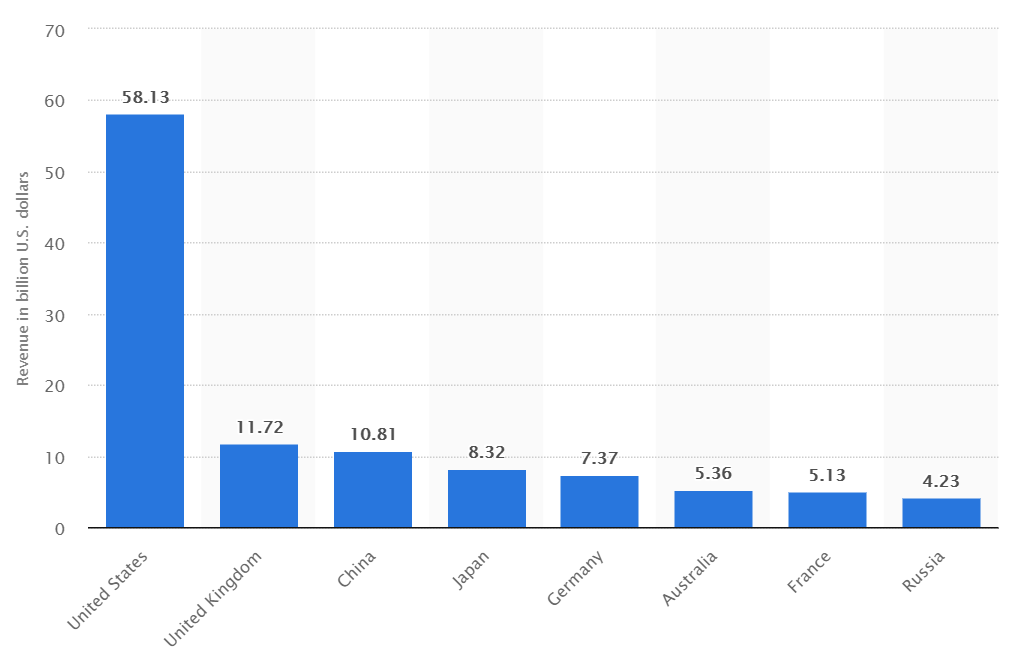
\includegraphics[height=6.2cm]{largestOnline2017}
\caption{Largest online advertisement markets in 2017. \cite{largest2017}}
\label{fig:largestOnline2017}
\end{figure}
Overall, the European online ad market grew by 12.3 percent in 2016 on 2015. The fastest growing online advertising markets that year were Slovenia and Ireland. 

In the United Kingdom, online advertising expenditures increased by nearly five billion British pounds between 2007 and 2015, from 2.81 billion British pounds to 7.71 billion British pounds \cite{europe2017}. Paid search and display advertising accumulated the highest share of spending. Google's net digital advertising revenue was the highest in the UK and is projected to grow further in future years. While Google generated more than 2.5 billion British pounds in revenue through its digital advertising channels in 2013, Facebook’s digital ad revenue accounted for 371 million British pounds.

In the U.S., the first quarter of 2017 marked the highest ever Q1 earnings for online advertising, at \$19.6B, according to the latest IAB Internet Advertising Revenue Report by the Interactive Advertising Bureau (IAB) and prepared by PwC US. These numbers show the increasing amount of revenue generated by online advertisement and why they are so crucial to industries and businesses across the world.

In Germany, the 2017 revenues stood at \$7.37B. This number is expected to grow to \$8.40B by 2020 and to \$9.21B by 2022. The major revenue categories ranked by percentage shares are as follows:
\begin{itemize}
	\item Search Advertising with \$3.44B - 48\%
	\item Banner Advertising with \$1.46B - 20.5\%
    \item Classified Advertising with \$0.95B - 13\%
    \item Social Media advertising with \$0.89B - 12.5\%
    \item Video Advertising with \$0.40B - 6\%
\end{itemize}

\textbf{The popularity of ad-blockers.} The issues with online ads have resulted in the increasing usage of ad-blocking software. Ad-blocking software (or ad-blocker) is an effective tool that blocks ads seamlessly, generally published as extensions in web browsers such as Chrome and Firefox. The soaring popularity of ad-blockers now mean that mobile Ad-block usage has surpassed desktop Ad-block usage. The total number of devices that use Ad-block encompassed 615 million devices by 2016 end \cite{popularity2017}. Some of the top reasons to use ad-blockers include security, interruption, website load time, too many ads or privacy issues. In a survey of U.S. demographics, men were 34\% more likely to use ad-blockers than women on desktop and laptop computers. Suburban and urban internet users were 17\% more likely to install ad-blockers than those in rural areas.

\textbf{The popularity of ad-blockers in Germany.} According to PageFair statistics \cite{popularity2017}, Germany ranked highest in Ad-block penetration when it came to desktop ad-blockers (Figure \ref{fig:popGermany}). \begin{figure}
\centering
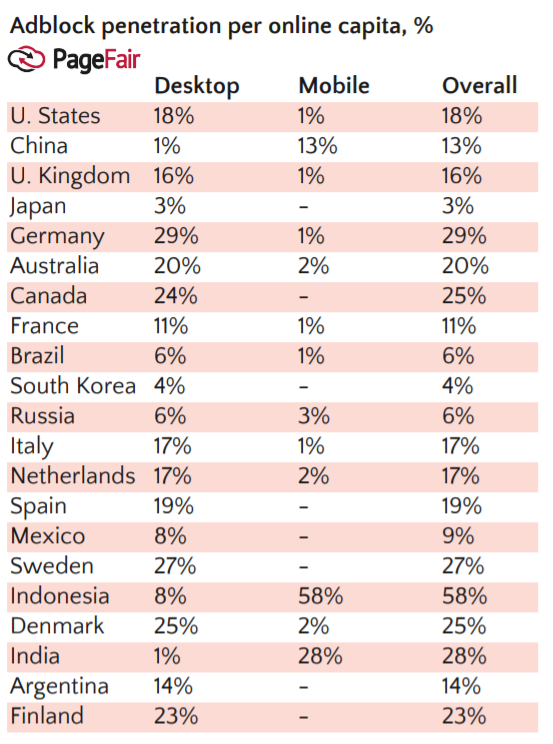
\includegraphics[height=6.2cm]{popGermany}
\caption{Top Ad Markets (ad spend) statistics.}
\label{fig:popGermany}
\end{figure}
These statistics indicate a tremendous potential for European markets since there is no clear single solution for mobile Ad-block usage. Legacy desktop Ad-block installations are not yet being replaced with mobile equivalents and as such the first mobile Ad-block solution to gain traction in Europe will connect with a large audience of former desktop Ad-block users.

On the contrary, a report by Bundesverband Digitale Wirtschaft (BVDW) and Online-Vermarkterkreis (OVK) titled  "Zentrale Adblocker-Rate des OVK" \cite{declineGermany} in December, 2016 showed a dip in ad block incidence rates from Q1 to Q3 of 2016 (Figure \ref{fig:declineGermany}). \begin{figure}
\centering
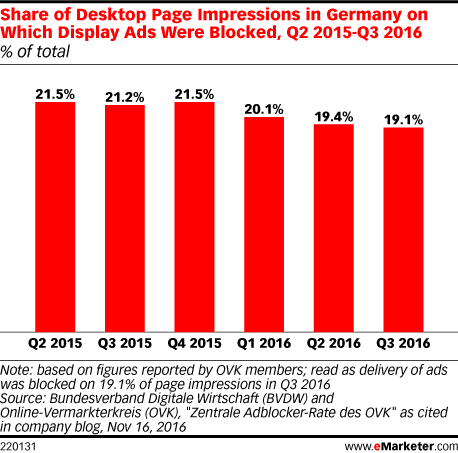
\includegraphics[height=6.2cm]{declineGermany}
\caption{Top Ad Markets (ad spend) statistics.\cite{declineGermany}}
\label{fig:declineGermany}
\end{figure}

The critical difference to be noted in the two sources cited above is that PageFair looked at the number of penetration/installations of ad-blockers while BVDW \& OVK focused on the actual number of websites that were affected by such ad-blockers.

\textbf{Economic Impact of Ad-blocking.} Ad block usage in the United States resulted in an estimated \$5.8B in blocked revenue during 2014 \cite{costBlock}. It had been estimated to cost \$10.7B in 2015 and \$20.3B in 2016. With the ever increasing number of Ad-block users the global cost of ad blocking surpassed the projected numbers of \$40B in 2016 making it crucial for the understanding of the effects of Ad-block on the economy.

\textbf{How do ad-blockers work?} Ad-blockers remove
ads by either page element removal or web request blocking. For web request blocking, ad-blockers look for certain URLs and remove the ones that belong to advertisers. For page element removal, ad-blockers use various CSS selectors to access elements and end up removing them. For both of these actions, ad-blockers are dependent on filter lists that contain the set of rules (as regular expressions) specifying the element selectors and domains to remove. There are various kinds of filter lists available which can be included in ad-blockers. Each of these lists serves a different purpose. For example, Adblock Plus by default includes EasyList \cite{easyList}, which provides rules for removing ads from English websites. EasyPrivacy \cite{easyPrivacy} helps ad-blockers to protect user privacy by removing trackers.

\begin{figure}
\centering
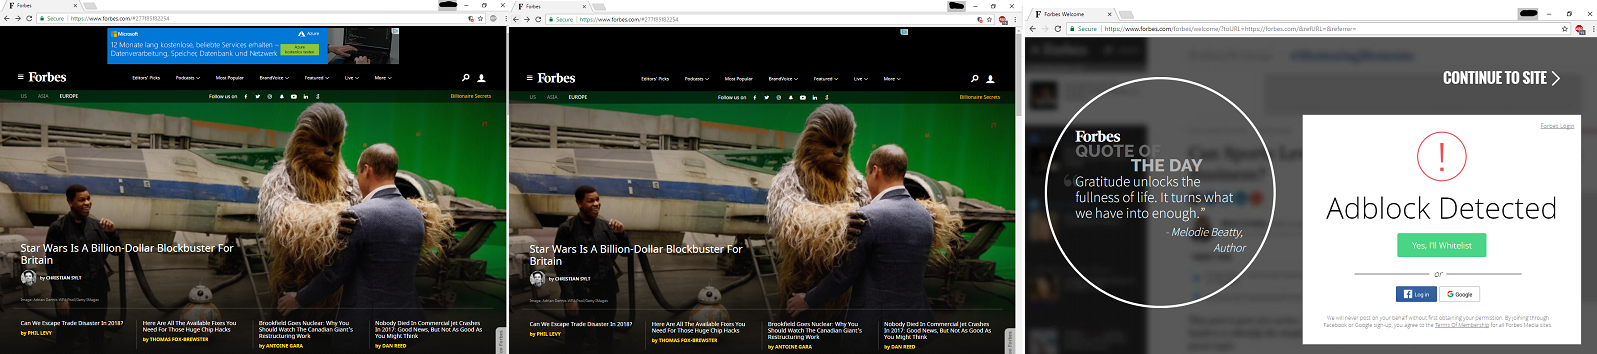
\includegraphics[height=2.8cm]{forbes}
\caption{Web page evolution for Forbes shows from left to right web page with ads, with ad-blocker enabled and with an Anti Ad-blocker.}
Source: \url{www.forbes.com}
\label{fig:forbes}
\end{figure}

Listing \ref{listing:adShow} shows ad code for display on the website:
\begin{listing}[!h]
\begin{minted}[mathescape,
               linenos,
               numbersep=5pt,
               frame=lines,
               baselinestretch=1.2,
			   fontsize=\footnotesize,
               escapeinside=||,
               framesep=2mm]{js}
               
<script>
   try {
   	fbs_settings.blocked_classes = ["sidebar_ADBOX","textlinkads",
          "advertisement-banner","externalAdComponent","ad_label2a",
          "adseparator","content-advertisment","review_ad1","loop-ad",
          "BottomGoogleAds","ad-160-160","aopsadvert","sidebar_advertising",
          "yan-sponsored","advertBox","ad-parent-hockey","block-maniad",
          "advertising-block","google_ad_wide","txtAd","rightSideSponsor",
          "adwolf-holder","view-display-id-ads_all","ad_links",
          "advertisement-tag","widget_ad_rotator","ad-caption",
          "ads-bottom-block","gemini-ad","rightColAdBox"];} 
   catch(err) {
   	fbs_settings.blocked_classes = null;
   }
</script>
<script type="text/javascript">setTimeout(function() {
   document.getElementById('main-content').className = '';
   }, 1000);
   try {
   performance.mark('blocking_scripts_start');
   } catch (e) {}
</script>
<script src="//i.forbesimg.com/forbes/scripts/b4b56484.vendor.js"></script>
<script src="//i.forbesimg.com/forbes/scripts/0d9abc37.scripts.js"></script>
<div id="css-js-dynamic"><span class="dynamic-css">false</span>
   <span class="dynamic-js"></span>
</div>
<div ng-if="!$root.is_mobile" id="teconsent"></div>
<script>$(window).on("touchstart", function(e){});</script>
<script type="text/javascript">
   try {
   	performance.mark('blocking_scripts_end');
   	} catch (e) {}
</script>
\end{minted}
\caption{Script to show how an ad is displayed on the website}
\label{listing:adShow}
\end{listing}

Listing \ref{listing:adBlockDetection} shows code how the ad-blocker is detected on the website's JavaScript code:
\begin{listing}[!h]
\begin{minted}[mathescape,
               linenos,
               numbersep=5pt,
               frame=lines,
               baselinestretch=1.2,
			   fontsize=\footnotesize,
               escapeinside=||,
               framesep=2mm]{js}
               
j = document.createElement("div"),
j.setAttribute("class", r.join(" ")), 
document.body.appendChild(j), "none" === window.getComputedStyle(j).display 
&& (this.removeWelcomeCookies(), this.adblock_state = "on")
}
}, this.removeWelcomeCookies = function() {
        var b = function() {
            s = !0, window.advBidxc && advBidxc.adBlockDetected 
            || window.uabfunc && window.uabfunc.detected 
            || (a.remove("welcomeAd", {
                path: "/",
                domain: ".forbes.com"
            }), a.remove("dailyWelcomeCookie", {
                path: "/",
                domain: ".forbes.com"
            }), a.put("re_ab", 1, {
                path: "/",
                domain: ".forbes.com"
            }))
        };
\end{minted}
\caption{Script to show how an ad-blocker code is detected on a website's Javascript code}
\label{listing:adBlockDetection}
\end{listing}
Ad-blockers also work on the following two techniques:

\textit{Filter Lists:} FilterLists \cite{filterLists} helps to protect privacy and security when using the Internet. It provides a comprehensive directory of subscription lists to block advertisements, malware, trackers, and other general annoyances. As users browse the Internet, they compare HTTP requests to their list of hosts and filters to selectively block advertisements, trackers, and general annoyances. This filtering helps to protect the surfer’s privacy, prevents malware attacks, and reduces bandwidth requirements.

\textit{Filter Matching:} Usually Adblock Plus treats filters as if it had a wildcard at its beginning and end, e.g. there is not difference between the filters ad and *ad*. Sometimes we want the filter to only match at the beginning or the end of an address. In such a case, Adblock Plus has come up with a solution that uses a pipe symbol to skip or start from any particular point in a website's URL \cite{filterMatching}.

\textbf{Ad-blocker extensions.} The following are the most common ad-blocker extensions used in desktop and mobile browsers based on ratings and number of downloads:
\begin{itemize}
\item $\mu$Block Origin for Chrome and Firefox
\item AdBlock for Chrome
\item Adblock Plus for Firefox, Chrome, Opera and Safari
\item AdBlock Pro for Chrome
\item Adguard for Chrome and Firefox
\item AdRemover for Chrome
\item Ghostery for Chrome, Firefox, Opera, Safari, Internet Explorer, Android and iPhone iOS
\item Simply Block Ads! for Chrome
\item SuperBlock AdBlocker for Chrome
\item $\mu$ Adblock for Firefox
\item uMatrix for Firefox, Chrome and Opera
\end{itemize}

\textbf{The rise of Anti Ad-blockers.} The online advertising industry considers such ad-blockers as a threat to their business models which revolves heavily around advertisements. This has led to a strong conflict between publishers and ad-blocking tools. IAB's script "DEAL"s (Detect, Explain, Ask, Limit) with such ad-blockers \cite{IAB2017}. Such scripts help publishers detect ad-blockers in browsers when users visit their websites (detection). Once detected, publishers ask
users to turn off their ad-blocking tool. These can range from a small message on the website to more aggressive blocking of website content and/or functionality. 

\begin{figure}
\centering
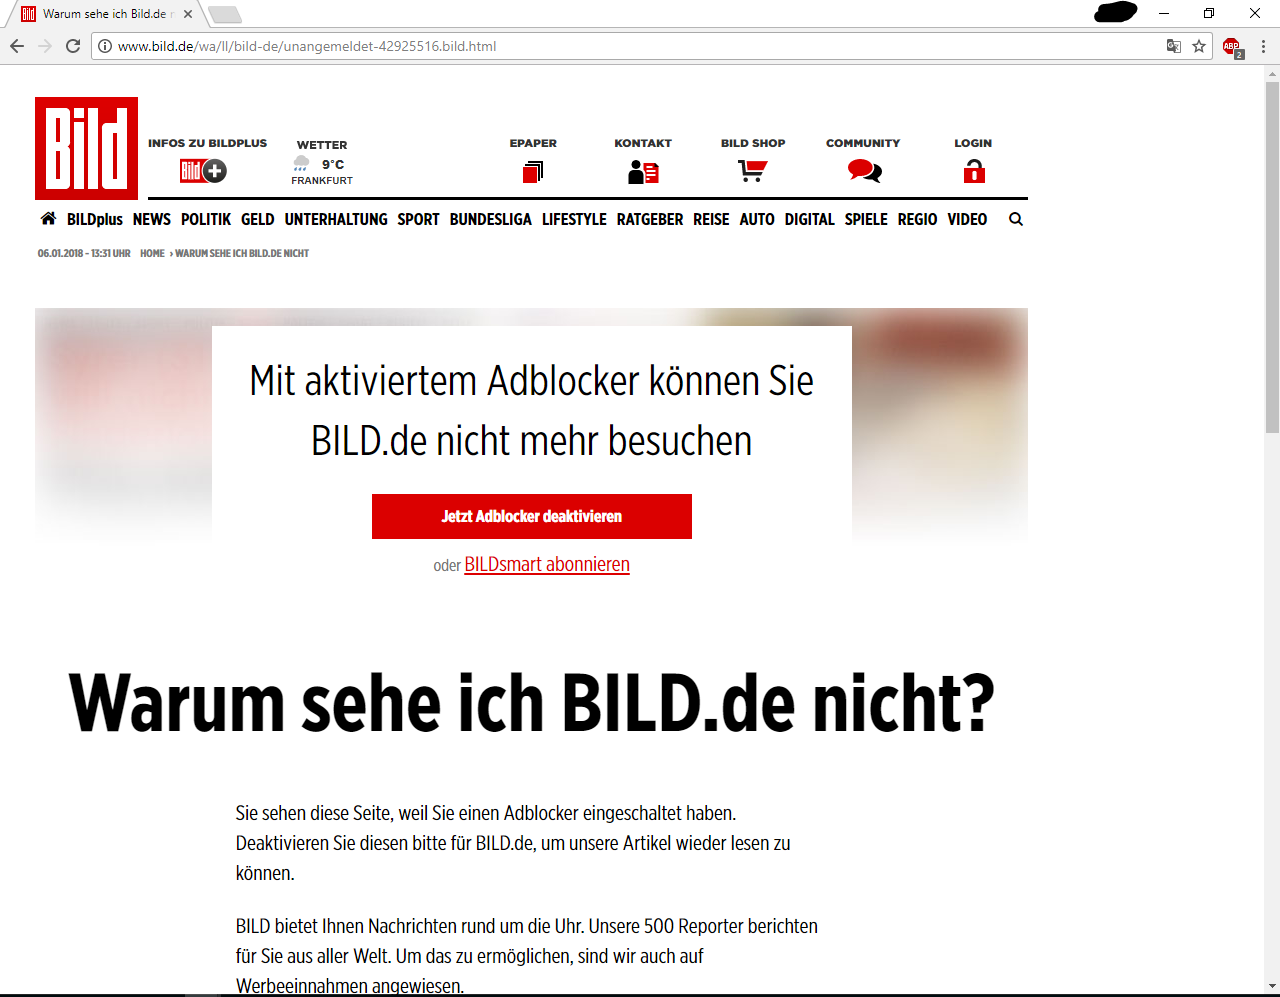
\includegraphics[height=4.0cm]{bildde}
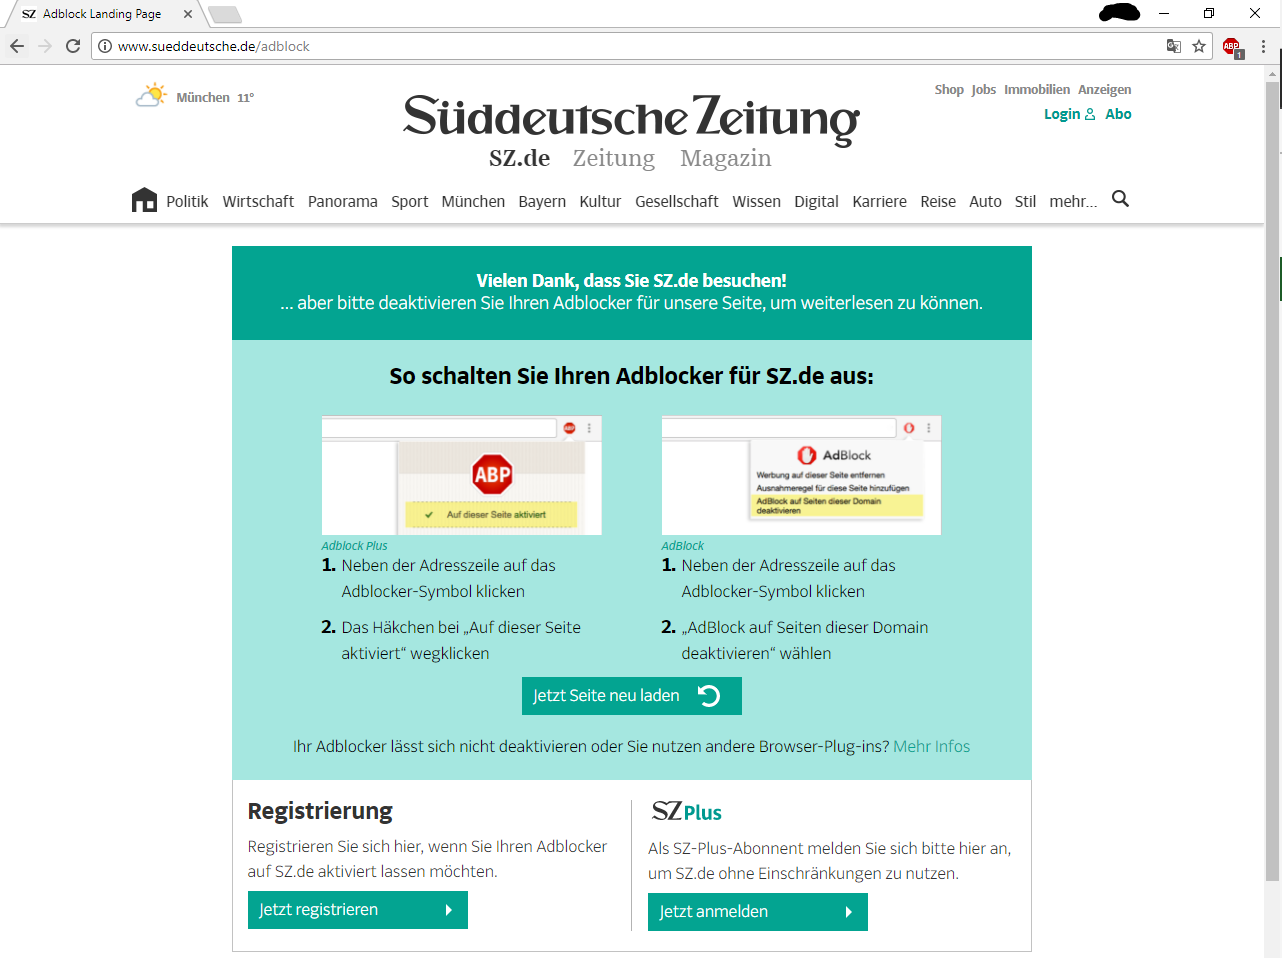
\includegraphics[height=4.0cm]{suedzeit}
\caption{German websites using ad-blocker detection scripts.}
\label{fig:germanBlocks}
\end{figure}

Figure \ref{fig:germanBlocks} shows a couple of examples of ad-block detection responses. This is done by employing Anti Ad-blocking tools or scripts that detect the usage of such ad-blockers. When a user with the ad-blocking tool opens such a website, these scripts typically identify if any ads have their visibility altered. If ads are found hidden or removed by an ad-blocker, publishers take countermeasures according to their policies.

\textbf{Impact of Anti Ad-blockers.} Around 9\% of today's most popular websites \cite{Shitong2017} deploy Anti Ad-blocker scripts to fight off the usage of ad-blockers that generate significant advertising revenues. Researchers at the University of Iowa and University of California-Riverside scanned Alexta Top 5K websites for anti Ad-block tools Anti Ad-block Killer List \cite{aakl} and Combined EasyList for anti Ad-block scripts. The results (Figure \ref{fig:anti-study}) showed a gradual increase in Anti Ad-blocking scripts, that prove the online advertising industry reacting to the immediate losses incurred by the use of ad-blockers on their websites.

\begin{figure}
\centering
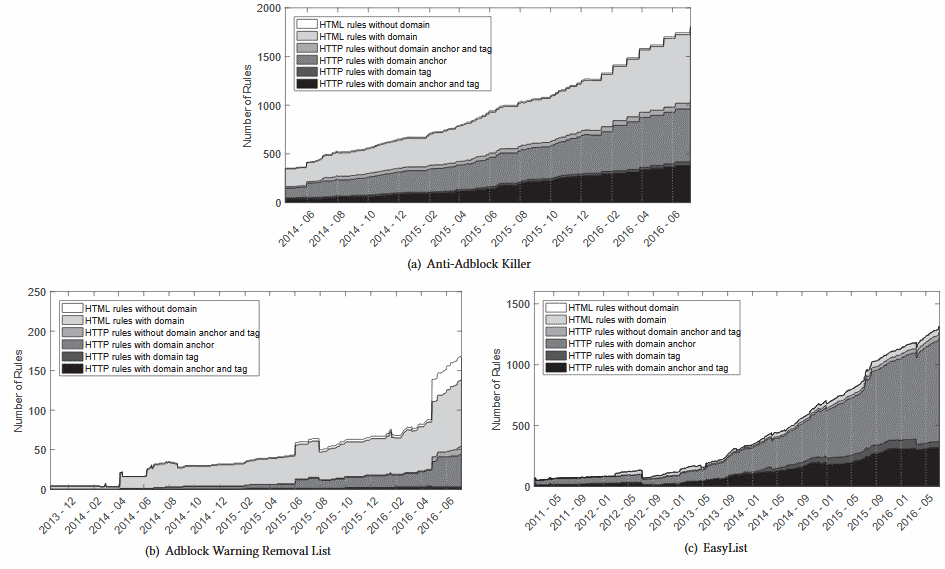
\includegraphics[height=6.2cm]{anti-study}
\caption{Anti Ad-blocking scripts with their gradual rise in usage \cite{popAnti2018}}
\label{fig:anti-study}
\end{figure}

When it comes to economy, ad-block usage in the United States resulted in an estimated \$5.8B in blocked revenue during 2014 \cite{costBlock}. These numbers are expected to grow to \$60B in 2018 making it crucial for businesses, industries and publishers to deploy Anti Ad-blockers.

\textbf{Economic impact of ad-blockers on browser performance and page load times.} In an extensive analysis on browser performance and page load times, Kiran et al.  \cite{Kiran2017} conclude that (i) uBlock has the best performance, in terms of ad and third party tracker filtering, and least privacy tracking, (ii) the time to load pages is not necessarily faster when using ad-blockers, and (iii) this is partly the case due to additional trackers and libraries being introduced by the ad-blocking tools.

\subsection{Related Work}
\textbf{Online Advertising.} Online advertising has emerged as one of the main sources of revenue on the web \cite{largest2017}. While advertisers claim
that ads on the web help keep most parts of the web free for consumers, consumers find advertising annoying
and potentially dangerous. Moreover, many users perceive such ads as a threat to privacy and tracking making it an important reason to install ad-blockers \cite{popularity2017}. Yu et al. \cite{Yu2016} found that 95\% of the pages visited contain 3rd party requests to potential trackers and 78\% attempt to transfer unsafe data. Ad-blockers also remove tracking buttons (such as Facebook’s ‘like’ button) and protect their users
from known malware domains.

\textbf{Ad-blockers.} The topic of ad-blockers have encouraged researchers to study it's usage and effects. Pujol et al. conducted a measurement study using passive network traces of thousands of users from a European ISP to quantify ad-block usage \cite{Pujol2015}. Their
results show that 22\% of users use AdBlock Plus. They
also found that ad-block users still generate significant
ad traffic due their enrollment in the acceptable
ads program. They also found little evidence that Adblock Plus users install the EasyPrivacy \cite{easyPrivacy} list of filters, which aims to protect end users’ privacy by blocking trackers. Also, they concluded that Adblock Plus users are mostly interested in blocking annoying ads rather than protecting their privacy, or that they are not aware of these options or how to change them.

\textbf{Anti Ad-blockers.} Our paper discusses in length the Anti Ad-blocking techniques and their effects adopted by Nithyanand et al. \cite{Rishab2016} and Haris et al. \cite{Haris2015}. Nithyanand et al. \cite{Rishab2016} clustered JavaScript snippets and manually analyzed these
clusters to identify third-party Anti Ad-blockers. They
found that 6.7\% of top 5K Alexa websites employ anti
ad-blockers. They also consider all websites that include Anti Ad-block scripts in their analysis. Haris et al. \cite{Haris2015} observed that at least 686 websites in the Alexa top-100K currently deploy Anti Ad-blockers at their home page to detect ad-block users and respond with visible notifications. The notifications ask users to either disable ad-blockers, consider donation, or pay a subscription fee. Such notifications cannot be disabled unless users disable ad-blockers or pay up. These could potentially harm their business. To counter such Anti Ad-blockers, ad-blockers now use filter lists to
remove Anti Ad-block scripts and ad-block detection
warnings. EasyList \cite{easyList}, which is used by ad-blockers to block ads, now contains rules that specifically target Anti Ad-blockers. Anti Ad-block Killer
list \cite{aakl} mostly contains web request blocking rules to remove Anti Ad-block scripts. The rules in these independently run crowd-sourced lists are tailored to specific Anti Ad-blockers.

\section{Detecting Anti Ad-blockers}

\subsection{Overview}
    
\subsection{Methodology}
    
\textbf{Crawler overview}
        
            Img
            
\textbf{A/B testing}
        
            Img
            
\textbf{Browser profiles}
        
\textbf{Identifying JS objects with common sources}
        
            code
            
\textbf{Choice of similarity metric and threshold}
        
\textbf{Improving scalability}
        
\textbf{Source and functionality identification}
        
\textbf{Method limitations}
        
\section{Datasets and Results}

\subsection{Characterizing websites that employ Anti Ad-blocking}
    
\subsection{Comparison of different ad-blockers and profiles}
    
\subsection{Website response to detection of Ad-blockers}
    
\subsection{Geographical Comparison}
    
\subsection{Limitations}
    
\section{Discussion}

\subsection{How Anti Ad-blockers work: Analyzing Anti Ad-blocker scripts}

Anti Ad-blocker scripts perform two basic operations (1) detect the presence of ad-block plugins (2) display a message asking the user to either disable ad-block or to whitelist the website or silently track the usage of the ad-blocker and report back to a server. These scripts employ a wide variety of tactics to achieve this. These may range from using simple scripts from first-party domains which check display-related attributes e.g. height, width of ads to detect ad-blockers to more sophisticated scripts from third-party domains that provide baits, do continuous detection, use cookies to track ad-block detection across various visits. These scripts are usually highly obfuscated and use different mechanisms so it becomes a challenge to detect and understand them.

\textbf{Collecting scripts}

To be filled. TBA.

\textbf{First-Party Anti Ad-blocking scripts}

Listing \ref{listing:antiAdBlockCode} shows a simple first-party ad-blocking script taken from a real-world website. They rely mostly on a bait.

\begin{listing}[!h]
\begin{minted}[mathescape,
               linenos,
               numbersep=5pt,
               frame=lines,
               baselinestretch=1.2,
			   fontsize=\footnotesize,
               escapeinside=||,
               framesep=2mm]{js}
               
<div class="banner_ads">&nbsp;</div>
<script>
var ads = document.getElementsByClassName('banner_ads'),
ad = ads[ads.length - 1];
if (!ad || ad.innerHTML.length == 0 || ad.
clientHeight === 0)
alert("We’ve detected an ad blocker running on
your browser." + ...);
}
</script>
\end{minted}
\caption{A simple Anti Ad-blocking example from a real website}
\label{listing:antiAdBlockCode}
\end{listing}

\textit{Timing:} These scripts typically work on page load but may add a delay of a few seconds using setTimeInterval(). The aim is to wait for the ad-blocker to remove the ads before trying to detect them.

\textit{Detection Logic:} We note that the Anti Ad-blocking script injects an empty div whose class is set to banner\_ads which is a known class type that will trigger blocking. This is the bait. The code then simply checks whether the ad frame is blocked to determine the presence of ad-blockers. Specifically, when an ad-blocker is used, the ad frame will become undefined, and its length and height values will be zero. The if condition in the Anti Ad-blocking script checks the values of these attributes. If the script detects that the value of either of these attributes is zero, it detects ad-blocker and reacts by displaying an alert and subsequently redirecting the user to a subscription page (code omitted for brevity). Without ad-blocker, the if condition will not be satisfied.

\textit{Response:} To be filled. TBA.


\textbf{Third-Party Anti Ad-blocking scripts}

Now we take a look at third-party ad-blocking scripts. These are more sophisticated than the First-Party techniques and employ several detection techniques at the same time. They also provide options to customize messages seen by the user and the action that the user has to take.

\begin{listing}[!h]
\begin{minted}[mathescape,
               linenos,
               numbersep=5pt,
               frame=lines,
               baselinestretch=1.2,
			   fontsize=\footnotesize,
               escapeinside=||,
               framesep=2mm]{js}
var e = {
         adblock: "chrome-extension://gighmmpiobklfepjocnamgkkbiglidom/
         	img/icon24.png",
         adblock_plus: "chrome-extension://cfhdojbkjhnklbpkdaibdccddilifddb/
         	block.html",
         adblock_pro: "chrome-extension://ocifcklkibdehekfnmflempfgjhbedch/
         	components/block/block.html",
         adblock_premium: "chrome-extension://fndlhnanhedoklpdaacidomdnplcjcpj/
         	img/icon24.png",
         adblock_super: "chrome-extension://knebimhcckndhiglamoabbnifdkijidd/
         	widgets/block/block.html",
         adguard: "chrome-extension://bgnkhhnnamicmpeenaelnjfhikgbkllg/
         	elemhidehit.png",
         adremover: "chrome-extension://mcefmojpghnaceadnghednjhbmphipkb/img/
         	icon24.png",
         ublock: "chrome-extension://epcnnfbjfcgphgdmggkamkmgojdagdnn/
         	document-blocked.html"
         }

\end{minted}
\caption{Identifying installed extensions}
\label{listing:extensions}
\end{listing}
            
\textit{Timing:} PageFair script performs periodic checks at various times of pageLoad to detect ad-blockers.

\textit{Detection Logic:} PageFair detects ad-blockers by looking for various extension resources (as shown in Listing \ref{listing:extensions}) exposed by popular ad-blockers like adblock, adguard, adremover and ublock at chrome-extensions://. Each ad-blocker has an unique extension identifier. It also uses multiple baits (Listing \ref{listing:multiBaits}) such as divs whose id is set to an identifier which is blocked by ad-blocker. The second method is a script bait where it tries to download a script "adsense.js".

\begin{listing}[!b]
\begin{minted}[mathescape,
               linenos,
               numbersep=5pt,
               frame=lines,
               baselinestretch=1.2,
			   fontsize=\footnotesize,
               escapeinside=||,
               framesep=2mm]{js}
               
            function v(a, e, d) {
                var b = document.createElement("DIV");
                b.id = d;
                b.className = e;
                b.style.width = "1px";
                b.style.height = "1px";
                b.style.top =
                    "-1000px";
                b.style.left = "-1000px";
                document.body.appendChild(b);
                e = jQuery("#" + d);
                d = e.is(":hidden") ? 1 : 0;
                q[a + "_hid_t0"] = c.browser.mozilla ? 0 : d;
                e.remove();
                g()
            }

            function d(a) {
                function e(a) {
                    var b = c.m(q);
                    0 < c.t(b, "s_blk") || (b = jQuery("#" + d), q.s_blk = a, b.remove(), g())
                }
                var d = c.j(),
                    b = document.createElement("SCRIPT");
                9 > c.J || c.browser.safari || c.browser.mozilla ? setTimeout(function() {
                    e(0)
                }, 1) : (c.d(b, "load", function() {
                    e(0)
                }), c.d(b, "error", function() {
                    e(1)
                }));
                b.id = d;
                b.type = "text/javascript";
                document.getElementsByTagName("head")[0].appendChild(b);
                b.src = a
            }
\end{minted}
\caption{Multiple baits and timeout}
\label{listing:multiBaits}
\end{listing}

\textit{Response: } To be filled. TBA.



\textbf{Community Anti Ad-blocking scripts}

Code:  To be filled. TBA.

\textit{Timing:} To be filled. TBA.

\textit{Detection Logic:} To be filled. TBA.

\textit{Response:} To be filled. TBA.

\subsection{Anti Ad-blocker suppliers}
To be filled. TBA.

\subsection{Ad-blocker response to being blocked}
To be filled. TBA.

\textbf{Anti Ad-block filter lists}
To be filled. TBA.

\textbf{Comparative Analysis of Anti Ad-block Lists}
To be filled. TBA.
Add Graph : To be filled. TBA.

\section{Alternatives to Anti Ad-blocking}
\subsection{Acceptable Ads}
Acceptable ads programme (by Adblock Plus) lays down a technique that is focussed on effecting ads on websites. They define a certain set of criterias that ensure that ads placed on websites are not annoying to users, distrupt or distort the web page content and are transparent such that there are no hidden ads or popups that violate the ad being accepted as an acceptable ad. The criterias \cite{accads} are defined as follows:

\textit{Placement:} Ads must be placed such that they do not disrupt the user's natural reading flow. Such ads must be inserted in the top, side or beneath the Primary Content. The Primary Content is either directly related or expands upon the central topic of a document or the central functionality of a software application.

\textit{Distinction:} Ads should not be mixed with any other content such that the user is misled into thinking of it as a primary content. Ads should be clearly marked with the word "Advertisement" or its equivalent.

\textit{Size:} Individual ad size requirements depend on the placement of the ad:\begin{itemize}
\item When placed above the primary content, the maximum height of an ad should be 200px.
\item When placed on the side of the primary content, the maximum width of an ad should be 350px.
\item When placed below the primary content, the maximum height of an ad should be 400px.
\end{itemize}

In addition to the above mentioned acceptable ads, there are various types or categories of ads that are not acceptable. They are listed as follows:
\begin{itemize}
\item Ads that visibly generate new ads if the Primary Content does not change
\item Ads with excessive or non user-initiated hover effects
\item Animated ads
\item Autoplay on sound or video ads
\item Ads that expand
\item Oversized image ads
\item Interstitial page ads
\item Overlay ads and overlay in-video ads
\item Pop-ups and Pop-unders
\item Pre-roll video ads
\item Rich media ads (e.g. Flash ads, Shockwave ads, etc.)
\end{itemize}

\subsection{WhiteLists}
Websites that adhere to the Acceptable Ads programme can apply for their websites to be whitelisted with Adblock Plus. This is very similar to anti-viruses marking some applications as "safe" and allowing them to run, while blocking other potentially harmful ones. As a common practice, publishers that detect ad-blockers ask users to whitelist their websites using the Disable or Whitelist option for the respective ad-blocker they are using. While most ad-blockers allow users to configure their browsers to whitelist individual websites, users rarely make use of this. That is where ad-blockers like Adblock Plus provide a default whitelist.

\subsection{User Perception}
Websites such as Forbes, request users to whitelist their site so that they can get "ad-light experience" for a few days. The Atlantic has started charging users for an ad-free version of their website if users do not disable ad-blockers. For users, it is about all or nothing.

\section{Anti Ad-block killers}
\subsection{How do they work} It tricks sites that use Anti Ad-blocker technology into thinking you aren’t using an Ad-blocker. The Ad-blocker blocker lets you keep your Ad-blocker on when you visit a page that would usually disable it by using a JavaScript file and filter list. This means you can work around bans on Ad-blockers from common news companies, like Forbes, which lock you out when you’re detected.

It works against a number of different technologies used to detect Ad-block users, and is likely to be a part of the next armsrace as publishers work out how to block the Ad-blockers using Ad-blocker blockers. 
Anti Ad-block killers like AAK \cite{AAK} are composed of a user script «AakScript» written in javascript and a filter list «AakList» using the same syntax as filter lists of AdBlock and AdBlock Plus. It helps one to keep Ad-Blocker active, when we visit a website and it asks us to disable. Script managers like Greasemonkey for Firefox or Tampermonkey for Chrome, Opera, Safari are necessary to install AakScript. Now AakList filter list can be added to Ad-block plugins like Adblock, AdBlock Plus, uBlock Origin or Adguard Blocker.

\section{Legality and Ethics of Anti Ad-blocking}
\subsection{Increasing Transparency}
The argument of Anti Ad-blocking ensues on the topic of maintenance of websites and henceforth businesses. Ad-block users often fail to understand how these websites pay for their monthly server and bandwidth charges. For most of such "free" sites, their revenue is generated through advertisements. Other websites use subscription services while the rest consume the costs. The latter ones are those that have another source of revenue which is usually not Internet based.

The bottom line of any business is that labor must be paid. It must be in accordance to what a writer, producer, musician, developer or any professional creates. This also revolves around the fact that the cost of living varies across the globe. Websites are compensated based on impressions measured by pay per click or cost per click on the adverts. While significantly bigger businesses could potentially hire more people to keep their websites running on profit, the smaller businesses are the ones who suffer the most. An analogy of going to a shop, purchasing an item and paying for the item collaborates with the model of advertisements. It is unethical to leave the shop without paying appropriately for the item. With the increasing cost of maintenance of websites and the cost of living, publishers rely heavily on such revenue sources.

There is a noticeable trend in publishers who detect the presence of ad-blockers are now fighting back against ad-blockers by asking users to disable ad-blockers or by subscribing for an ad-free version. This poses an ethical dilemma to users, using an ad-block and stopping revenue income for publishers as well as for publishers, using an Anti Ad-blocker to prevent users' intentions of blocking ads.

\subsection{Legality in European Union}

The Interactive Advertising Bureau (IAB) are of the opinion that ad block detection is not illegal. The European Commission had in a letter to privacy campaigner Alexander Hanff \cite{euHanff} specified that ad-blocker detection tool requires access to user data to determine if they have extensions or tools to block ads. Article 5.3 of the European Union's ePrivacy Directive \cite{eprivacy} states: "Member States shall ensure that the use of electronic communications networks to store information or to gain access to information stored in the terminal equipment of a subscriber or user is only allowed on condition that the subscriber or user concerned is provided with clear and comprehensive information in accordance with Directive 95/46/EC, inter alia about the purposes of the processing, and is offered the right to refuse such processing by the data controller. This shall not prevent any technical storage or access for the sole purpose of carrying out or facilitating the transmission of a communication over an electronic communications network, or as strictly necessary in order to provide an information society service explicitly requested by the subscriber or user."

Under this EU law, publishers must ask for permission before accessing a user's personal information, similar to how websites must ask for permission to store cookies on user devices. However the other side of the argument is that publishers are only detecting via Javascript if the ads have been delivered, not checking if any ad-blocker is installed, thus complying with the ePrivacy directive.

\subsection{Legality in Germany}

Media groups Süddeutsche Zeitung, Pro-Sieben-Sat.1, and IP Deutschland, an RTL subsidiary recently fought a legal battle against Cologne-based ad-blocking vendor Eyeo for banning of Eyeo's ad-blocking software Adblock Plus. The Munich higher regional court ruled \cite{wiredLegal} that the ad-blocking software Adblock Plus is legal. The Munich higher regional court also noted that the software did not violate any competition laws in Germany, with Eyeo’s business model not qualifying as "forbidden aggressive advertising". Although joining Eyeo's whitelist is free, the media groups are objecting to the fact that Eyeo is making money from the extra revenues that the advertisers are making by joining these whitelists under the Acceptable Ads programme.

This court order comes in contrast to another similar court order ruling in Cologne, where publisher Axel Springer secured a partial victory \cite{springerLoss} against Eyeo stating that Adblock Plus must add Axel Springer to the whitelist for free but must abide by the Acceptable Ads criteria. The constrast in such verdicts could potentially build up these cases to Germany’s Federal Court of Justice.

In a blog post detailing the court decisions \cite{adblockLegal} Adblock Plus maintain their legality under German laws and as such the German judges have since not favored the usage of ad-blocking detectors. 

In a Hamburg judgement for Spiegel versus Eyeo, which has since been made public, Eyeo cited \cite{hamburgJudgement} that as of August 2015, Adblock Plus was installed on approximately 9.55 million browsers with German IP addresses, which accounted for around 5\% of the computers in Germany used to access the Internet. Almost 3,500 websites were whitelisted for Adblock Plus' Acceptable Ads to be viewed by default. From these, around 90\% did not pay, but the largest 10\% did. The judges concluded that Internet users have a genuine interest in the removal of such undesired advertising, protection from potentially malicious softwares and control of their data.

\section{Conclusion} TBA
\subsection{Future Work} TBA
\subsection{Acknowledgements} TBA
\subsection{Source code and data release} TBA

















\begin{thebibliography}{x}

\bibitem{Haris2015} Haris Mughees, Muhammad, Qian, Zhiyun, Shafiq, and Zubair. Detecting Anti Ad-blockers in
the wild. proceedings on privacy enhancing technologies (2015)

\bibitem{Garimella2017} Garimella, Kiran, Kostakis, Orestis, Mathioudakis, and Michael. Ad-blocking: A study on performance, privacy and counter-measures (2017)

\bibitem{IAB2017} Interactive Advertising Bureau. Ad block detection code access request (2017) \url{https://
github.com/InteractiveAdvertisingBureau/AdBlockDetection}

\bibitem{Rishab2016} Rishab Nithyanand, Sheharbano Khattak, Mobin Javed, Narseo Vallina-Rodriguez, Marjan
Falahrastegar, Julia E. Powles, Emiliano De Cristofaro, Hamed Haddadi, and Steven J. Murdoch. Ad-blocking and counter blocking: A slice of the arms race (2016)

\bibitem{TechCrunch2016} Tech Crunch. Blocking ad blockers boosted facebook’s desktop ad revenue 18 percent (2016) \url{https://techcrunch.com/2016/11/02/add-cash-plus}

\bibitem{Barford2014} Barford, P., Canadi, I., Krushevskaja, D., Ma, O., Muthukrishnan, S.: Adscape:
harvesting and analyzing online display ads. In:  Proceedings of the 23rd International Conference on World Wide Web, pp. 597-608 (2014)

\bibitem{Gill2013} Gill, P., Erramilli, V., Chaintreau, A., Krishnamurthy, B., Papagiannaki, K., Rodriguez, P.: Best paper - follow the money: understanding economics of online aggregation and advertising. In: Proceedings of the 2013 Conference on Internet Measurement Conference, IMC 2013, pp. 141-148  (2013)

\bibitem{Mayer2012} Mayer, J.R., Mitchell, J.C.: Third-party web tracking: policy and technology. In: 2012 IEEE Symposium on Security and Privacy (SP), pp. 413–427 (2012)

\bibitem{Castelluccia2012} Castelluccia, C., Kaafar, M.-A., Tran, M.-D.: Betrayed by your ads!. In: Fischer-
Hubner, S., Wright, M. (eds.) PETS 2012. LNCS, vol. 7384, pp. 1–17. Springer, Heidelberg (2012)

\bibitem{Datta2015} Datta, A., Tschantz, M.C., Datta, A.: Automated experiments on ad privacy settings. Proc. Priv. Enhanc. Technol. 2015(1), 92–112 (2015)

\bibitem{Google2018} Google chrome adblock plus. https://chrome.google.com/webstore/detail/adblock-plus/cfhdojbkjhnklbpkdaibdccddilifddb/support?hl=en-GB

\bibitem{Pujol2015} Pujol, E., Hohlfeld, O., Feldmann, A.: Annoyed users: ads and ad-block usage in the wild. In: Proceedings of the 2015 ACM Conference on Internet Measurement Conference, pp. 93–106 (2015)

\bibitem{Apostolis2014} Apostolis Zarras, Alexandros Kapravelos, Gianluca Stringhini, Thorsten Holz, Christopher Kruegel, and Giovanni Vigna. The Dark Alleys of Madison Avenue: Understanding Malicious Advertisements. In Proceedings of the 2014 Conference on Internet Measurement Conference (IMC '14). ACM, New York, NY, USA, 373-380 (2014) \url{https://doi.org/10.1145/2663716.2663719}

\bibitem{europe2017} Digital advertising in Europe - Statistics and Facts (2017) \url{https://www.statista.com/topics/3983/digital-advertising-in-europe/}

\bibitem{largest2017} Online advertising revenue in major online advertising markets in 2017 (2017) \url{https://www.statista.com/statistics/246570/largest-online-advertising-markets/}

\bibitem{popularity2017} PageFair: 2017 Adblock Report (2017) \url{https://pagefair.com/blog/2017/adblockreport/}

\bibitem{declineGermany} Desktop Ad Blocking Continues Unexpected Decline in Germany (2016) \url{https://www.emarketer.com/Article/Desktop-Ad-Blocking-Continues-Unexpected-Decline-Germany/1014768?mod=djemCMOToday}

\bibitem{costBlock} The cost of ad blocking: PageFair and Adobe report (2015) \url{https://downloads.pagefair.com/wp-content/uploads/2016/05/2015_report-the_cost_of_ad_blocking.pdf}

\bibitem{easyList} EasyList. \url{https://easylist.to/easylist/easylist.txt}

\bibitem{easyPrivacy} EasyPrivacy. \url{https://easylist.to/easylist/easyprivacy.txt}

\bibitem{filterLists} Filter Lists. \url{https://filterlists.com/}

\bibitem{filterMatching} Matching filters through Adblock Plus. \url{https://adblockplus.org/filters#anchors}

\bibitem{popAnti2018} 9\% of Popular Websites Use Anti Ad-block Scripts (2018) \url{https://www.bleepingcomputer.com/news/technology/9-percent-of-popular-websites-use-anti-adblock-scripts/}

\bibitem{Shitong2017} Shitong Zhu, Xunchao Hu, Zhiyun Qian, Zubair Shafiq and Heng Yin. Measuring and Disrupting Anti Ad-blockers Using Differential Execution Analysis (2017)

\bibitem{Kiran2017} Kiran Garimella, Orestis Kostakis, and Michael Mathioudakis. Ad-blocking: A Study on Performance, Privacy and Counter-measures. In Proceedings of the 2017 ACM on Web Science Conference (WebSci '17). ACM, New York, NY, USA, 259-262 (2017) \url{https://doi.org/10.1145/3091478.3091514}

\bibitem{Yu2016} Zhonghao Yu, Sam Macbeth, Konark Modi, and Josep M Pujol. Tracking the Trackers. 121-132 (2016)

\bibitem{aakl} Anti AdBlock Killer List. \url{https://raw.githubusercontent.com/reek/anti-adblock-killer/master/anti-adblock-killer-filters.txt}

\bibitem{AAK} Anti Ad-block Killer \url{https://reek.github.io/anti-adblock-killer/}

\bibitem{accads} Acceptable Ads Criteria
\url{https://acceptableads.com/en/about/criteria}

\bibitem{euHanff} European Commission's letter to privacy campaigner Alexander Hanff
\url{https://twitter.com/alexanderhanff/status/722861362607747072}

\bibitem{eprivacy} Article 5.3 of the European Union's ePrivacy Directive (2002)
\url{http://eur-lex.europa.eu/legal-content/EN/TXT/?uri=CELEX:32002L0058}

\bibitem{wiredLegal} Adblock Plus: Werbeblocker bleiben in Deutschland legal (2017)
\url{https://www.wired.de/collection/business/gerichtsurteil-adblock-plus-verlage}

\bibitem{springerLoss} What Axel Springer’s loss in ad-blocking suit means for UK publishers (2016)
\url{https://digiday.com/uk/axel-springers-loss-ad-blocking-suit-means-uk-publishers/}

\bibitem{adblockLegal} Adblock Plus and (a little) more (2016)
\url{https://adblockplus.org/blog/it-s-still-perfectly-legal-to-block-ads-in-germany-after-latest-court-victory-over-spiegel}

\bibitem{hamburgJudgement} Urteil des Landgerichts Hamburg (Az. 315 O 293/15) (2016)
\url{http://www.landesrecht-hamburg.de/jportal/portal/page/bsharprod.psml?showdoccase=1&doc.id=JURE170021729&st=ent}







\end{thebibliography}
\end{document}
